\section{Depth-first search (DFS) \cite{ai/book/Artificial-Intelligence-A-Modern-Approach/Russell-Norvig}}
\label{AI: Algorithms/Depth-first search (DFS)}


\begin{figure}[H]
\centering
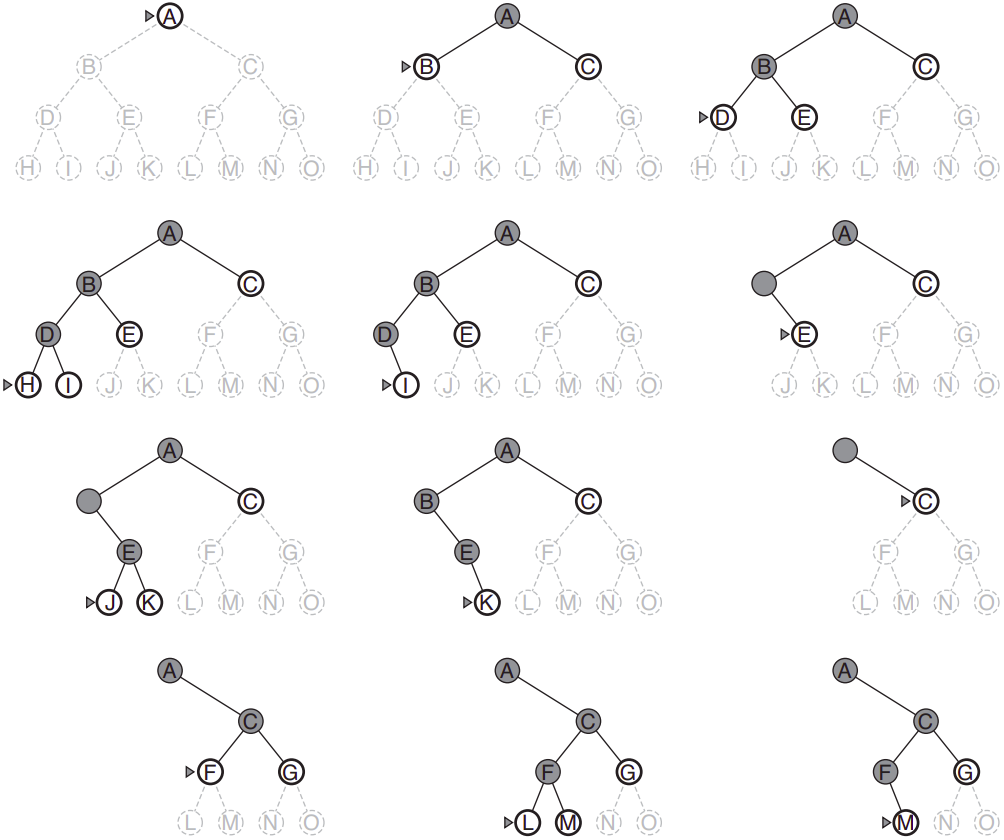
\includegraphics[
    width=\linewidth,
    height=7cm,
    keepaspectratio,
]{images/algorithms/Depth-first-search-illustration.png}
\caption*{
    Depth-first search on a binary tree. The unexplored region is shown in light gray. Explored nodes with no descendants in the frontier are removed from memory. Nodes at depth $3$ have no successors and $M$ is the only goal node. 
    \cite{ai/book/Artificial-Intelligence-A-Modern-Approach/Russell-Norvig}
}
\end{figure}


\begin{enumerate}
    \item Depth-first search always expands the \textbf{deepest node} in the current frontier of the search tree.
    \hfill \cite{ai/book/Artificial-Intelligence-A-Modern-Approach/Russell-Norvig}

    \item The search proceeds immediately to the deepest level of the search tree, where the nodes have no successors. As those nodes are expanded, they are dropped from the frontier, so then the search “backs up” to the next deepest node that still has unexplored successors.
    \hfill \cite{ai/book/Artificial-Intelligence-A-Modern-Approach/Russell-Norvig}

    \item \textbf{Performance}:
    \begin{enumerate}
        \item \textbf{graph-search version}:
        \begin{enumerate}
            \item \textbf{complete} in finite state spaces because it will eventually expand every node
            \hfill \cite{ai/book/Artificial-Intelligence-A-Modern-Approach/Russell-Norvig}

            \item \textbf{not optimal}
            \hfill \cite{ai/book/Artificial-Intelligence-A-Modern-Approach/Russell-Norvig}

            \item \textbf{time complexity}: $\mathcal{O}(b^d)$
            \hfill \cite{ai/book/Artificial-Intelligence-A-Modern-Approach/Russell-Norvig}

            \item \textbf{space complexity}: $\mathcal{O}(b^d)$
            \hfill \cite{ai/book/Artificial-Intelligence-A-Modern-Approach/Russell-Norvig}
        \end{enumerate}

        \item \textbf{tree-search version}:
        \begin{enumerate}
            \item \textbf{not complete}, as it can fall in \textit{infinite loop}
            \hfill \cite{ai/book/Artificial-Intelligence-A-Modern-Approach/Russell-Norvig}

            \item \textbf{not optimal}
            \hfill \cite{ai/book/Artificial-Intelligence-A-Modern-Approach/Russell-Norvig}

            \item \textbf{time complexity}: $\mathcal{O}(b^m)$
            \hfill \cite{ai/book/Artificial-Intelligence-A-Modern-Approach/Russell-Norvig}

            \item \textbf{space complexity}: $\mathcal{O}(bm)$
            \hfill \cite{ai/book/Artificial-Intelligence-A-Modern-Approach/Russell-Norvig}
        \end{enumerate}
    \end{enumerate}
\end{enumerate}


\subsection*{Implementation}

\begin{enumerate}
    \item The depth-first search algorithm is an instance of the graph-search algorithm that uses a LIFO queue.
    \hfill \cite{ai/book/Artificial-Intelligence-A-Modern-Approach/Russell-Norvig}

    \item  it is common to implement depth-first search with a recursive function that calls itself  on each of its children in turn. 
    \hfill \cite{ai/book/Artificial-Intelligence-A-Modern-Approach/Russell-Norvig}
\end{enumerate}

\begin{lstlisting}[
    language=Python,
    caption=Problem Solving Agent - Depth first search on a graph
]
from queue import LifoQueue

def depth_first_search(problem: Problem):
    node = Node(problem.initial_state, None, None, 0)

    if problem.goal_test(node.state):
        return solution(node)
    
    frontier = LifoQueue()
    explored = set()

    frontier.put(node)

    while True:
        if frontier.empty():
            return None
        
        node = frontier.get()
        explored.add(node)

        for action in problem.actions(node.state):
            child = child_node(problem, node, action)

            if (not any([n.state == child.state for n in frontier.queue]) and 
                not any([n.state == child.state for n in explored])):
                if problem.goal_test(child.state):
                    return solution(child)

                frontier.put(child)
\end{lstlisting}














